%doc settings
\documentclass[a4paper]{article}

%import packages
\usepackage[utf8]{inputenc}
\usepackage[czech]{babel}
\usepackage[total={15cm,25cm}, top=2cm, left=3cm, includefoot]{geometry}
\usepackage{amsmath,amsfonts,amssymb}
\usepackage{graphicx}
\usepackage{listings}
\graphicspath{{images/}}
\usepackage[figurename=Obr. ,justification=centering]{caption}

\lstdefinestyle{codestyle}{
	showstringspaces=false
}
\lstset{
	style=codestyle,
	aboveskip=15pt, 
	belowskip=12pt,
	breaklines = true,
	postbreak = \raisebox{0ex}[0ex][0ex]{\ensuremath{\hookrightarrow\space}}
}



\setlength{\parindent}{0pt}
\setlength{\parskip}{1em}

%about information
\newcommand{\enTitle}{LSTM NETWORKS}
\makeatletter
\title{LSTM SÍTĚ}\let\Title\@title
\author{Jakub Šťastný}\let\Author\@author
\makeatother
%document body
\begin{document}
\begin{titlepage}
	\centering
	\textbf{{\LARGE STŘEDOŠKOLSKÁ ODBORNÁ ČINNOST}}\par
	\vspace{0.5cm}
	\textbf{{\scshape\Large Obor SOČ: 18. Informatika}}\par
	\vfill
	\textbf{\LARGE \Title}\par
	\vspace{4cm}
	\textbf{\Large Autor: \Author}\par
	\vspace{1cm}
	\textbf{\Large Kraj: Jihomoravský}\par
	\vfill
	{\large Brno \the\year\par}
\end{titlepage}
\begin{titlepage}
        \centering
        \textbf{{\LARGE STŘEDOŠKOLSKÁ ODBORNÁ ČINNOST}}\par
        \vspace{0.5cm}
        \textbf{{\scshape\Large Obor SOČ: 18. Informatika}}\par
        \vfill
	\textbf{\LARGE \Title}\par\textbf{\Large \enTitle}\par
        \vspace{4cm}
        \textbf{\Large Autor: \Author}\par
        \vspace{1cm}
	\textbf{\Large Škola: Gymnázium Brno-Řečkovice, p. o.}\par
	\vspace{1cm}
        \textbf{\Large Kraj: Jihomoravský}\par
	\vspace{1cm}
	\textbf{\Large Konzultant: Mgr. Jan Herman}\par
        \vfill
	{\large Brno \the\year\par}
\end{titlepage}
\thispagestyle{empty}
${}$
\vfill
\section*{Prohlášení}
Prohlašuji, že jsem svou práci vypracoval samostatně a použil jsem pouze podklady (literaturu, projekty, SW atd.) uvedené v~seznamu vloženém v~práci SOČ. Prohlašuji, že tištěná verze a elektronická verze soutěžní práce jsou shodné. Nemám žádný důvod proti zpřístupňování této práce v~souladu se zákonem č. 121/2000 Sb., o~právu autorském, o~právech souvisejících s~právem autorským a o~změně některých zákonů (autorský zákon) v~platném znění.\par
v~Brně Dne \today \hfill Jakub Šťastný\par
\clearpage
\thispagestyle{empty}
${}$
\vfill
\section*{Poděkování}
Děkuji Mgr. Janu Hermanovi za veškerou pomoc, kterou mi během práce poskytl. 
\clearpage
\thispagestyle{empty}
\section*{Anotace}
Práce se zabývá neuronovými sítěmi a to konkrétně architekturou LSTM (Long-short term memory). Neuronové sítě jsou velmi používaným nástrojem v~oboru strojového učení a umělé inteligence. Nacházejí uplatnění ve spoustě oborech a to hlavně tam, kde není potřeba anebo dokonce nelze znát 100\% přesný výsledek a ostatní algoritmy nejen z~časových důvodů selhávají. V~teoretické části práce jsem popsal základní fungování neuronových sítí architektury LSTM. V~praktické části jsem použil nabytých znalostí k~vývoji vlastní sítě, sloužící k~predikci následujícího znaku během generování textu.\par
Klíčová slova: Neuronové sítě; Long Short Term Memory; LSTM Sítě; umělá inteligence; strojové učení; generování textu, predikce následujícího znaku
\section*{Annotation}
The thesis deals with neural networks and with specific architecture LSTM (Long-Short Term memory). Neural networks are highly used tool in the field of machine learning and artificial intelligence. They are used in many fields of study, particularly where there is no need or even you can not know the 100\% exact result and where others algorithms fail not only because of time restrictions. In theoretical part of the thesis I~described the basic functionality of neural network architecture LSTM. In practical part I~often used the knowledge acquired to develop my own network used to prediction of next character during text generating.\par
Keywords: Neural networks; Long Short Term Memory; LSTM Networks; Artificial Intelligence; machine learning; text generating; prediction of next character
\newpage
\tableofcontents
\newpage
\section*{Úvod}
\addcontentsline{toc}{section}{Úvod}
Neuronové sítě jsou zásadním modelem strojového učení. Jedná se o~architektury, které nacházejí inspiraci v~biologii a to konkrétně v~nervové soustavě člověka a to především z~oblasti mozku. Jejich základní vlastností je to, že se dokáží na základě určitých dat samy učit problematice úkolu a získané znalosti dále zobecňovat na všechny možné příklady na základě podobností se vzorovými daty.\par
Tyto modely a algoritmy nacházejí uplatnění především v~situacích, kde není nutné a nebo i nelze znát stoprocentně přesný výsledek a kdy ostatní algoritmy nejen z~časových důvodů selhávají. Mezi příklady takovýchto situací patří například čtení rukou psaného textu, převod textu na řeč a naopak, rozpoznávání obrázků nebo také predikce časových řad, jako je například odhadování vývoje na burse.\par
V~teoretické části jsem se zabýval teorií fungování neuronových sítí architektury LSTM (Long-Short Term Memory). Dále jsem popsal architekturu této sítě a také algoritmus, který se využívá při jejím učení.
Praktická část se věnuje konkrétní implementaci LSTM sítě, která slouží k~predikci následujícího znaku textu a tím samotný text generuje.
\newpage
\begin{center}
\section{Úvod do neuronových sítí}
\end{center}
\subsection{Co jsou neuronové sítě}
Jde o~jeden z~typů výpočetních modelů používaný v~oboru umělé inteligence a strojového učení. Tyto sítě nacházejí inspiraci v~biologické struktuře nervové sítě a mozku, i když se tomuto vzoru již některé modely dosti vzdalují. Jde o~struktury, které mají schopnost učit se na základě dat podobného typu a následně na základě nabytých znalostí své postupy zobecňovat i na případy, které se v~množině učících dat vůbec nevyskytují.
\subsection{Biologická inspirace}
Jak jsem již psal, inspirací pro neuronové sítě se stala biologická nervová síť člověka. Ta je složena ze tří částí: mozku, míchy a samotných nervů. Nejsložitější a nejvýkonnější částí soustavy je bezpochyby mozek, který se právě snažíme ve tvorbě umělých sítí napodobit, i když nám převážně hardwarové podmínky neumožní se z~hlediska výkonu k~mozku ani zdaleka přiblížit. Základním stavebním článkem jak biologické tak umělé sítě je neuron, který má za úkol informaci, v~biologickém případě jí je elektrický impuls a v~případě umělé sítě reálné číslo, přijmout, určitým způsobem upravit a poslat ji dál. Biologické neurony přijímají signály pomocí dendritů, kterých obvykle bývá velká spousta, následně jej modifikují a výstup předávají dále pomocí axonu, který bývá právě jeden. Tomuto se opět velmi podobá i model umělých neuronů, jelikož opět v~drtivé většině modelů platí, že neurony přijímají více vstupů a generují právě jeden výstup. Neurony jsou jak v~biologické tak v~umělé struktuře spolu propojeny\footnote{tomuto spojení se také říká synapse} a navzájem si předávají informace, které každý neuron na základě svého úkolu upravuje a jsou tak schopny řešit i velmi složité problémy.
\subsection{Dělení neuronových sítí}
Existuje mnoho různých architektur, které klasifikujeme do několika tříd na základě některých společných vlastností. Jedním, asi nejdůležitějším, typem dělení je dělení na základě toho, jak v~síti proudí informace. Z~tohoto hlediska dělíme sítě na sítě dopředné a rekurentní, které ve své práci budu používat. Zatímco v~dopředných sítích proudí informace přímo dopředně v~systematické řadě, sítě rekurentní obsahují nějaký cyklus, tudíž v~ní data zůstávají i po vygenerování výstupu, tudíž obsahují nějakou paměť.\par
Dalším podstatným typem klasifikace neuronových sítí je podle způsobu učení a to na sítě, které se učí s~učitelem a bez učitele, s~tím, že ve své práci využiji typ sítí, které se učí s~učitelem. Rozdíl mezi těmito sítěmi je v~typu vstupních dat. Zatímco sítě, které se učí s~učitelem, mají vstupní data ve formě dvojic vstupu a předpokládaného výstupu, s~tím, že jejich učící algoritmus prožene vstup sítí, vygeneruje výstup, porovná jej se výstupem předpokládaným a následně na základě rozdílů upravuje synaptické váhy, kdežto sítě, které se učí bez učitele předpokládaný výstup k~datům nemají a jejich učící algoritmus se snaží hledat různé podobnosti mezi těmito daty.\par
Dále můžeme neuronové sítě dělit podle toho, k~čemu jsou určeny na sítě klasifikační, regresní a shlukovací. Výstupem sítí regresních bývá nějaké reálné číslo, které je počítáno na základě vstupu sítě. Sítě klasifikační mají jako možný výstup několik stavů, s~tím, že mají na základě vstupu rozhodnout pravděpodobnost toho, který stav je správný a který ne. Právě tento typ sítí ve své síti používám. Posledním typem je typ shlukovací, který shlukuje vstupy do více skupin na základě jejich společných vlastností a podobností.
\subsection{Použití neuronových sítí}
Neuronové sítě se používají především v~situacích, kdy není potřeba nebo naopak nelze znát stoprocentně přesný výsledek. Využití tedy nacházejí ve spoustě možných oborech a situacích, jako je čtení rukou psaného textu, převod textu na řeč a obráceně, predikce časových řad, jako třeba vývoj na burse, generování textu, básní písní, automatická úprava obrázků, určení diagnózy problému například v~medicíně a spousta dalších situací. To tedy znamená, že neuronové sítě jsou velmi mocným, rozšířeným a hlavně universálním nástrojem a je v~nich jistě velká budoucnost.
\begin{center}
\clearpage
\section{LSTM sítě}
\end{center}
\subsection{Architektura sítě}
 Tato část práce se zabývá architektonickou stavbou sítí LSTM. Snaží se čtenáři přiblížit, jak jsou sítě stavěné a jak v~nich proudí data nezávisle na procesu učení. Nejprve zde popíši dva druhy neuronových buněk a to perceptron a LSTM buňku\footnote{existuje samozřejmě mnoho dalších druhů neuronových buněk, ale tyto dvě jsou pro tuto práci podstatné}. Dále popíši, co je to neuronová vrstva a jak vypadá LSTM síť.
 \subsubsection{Perceptron}
Perceptron je nejjednodušší neuronová buňka, která má za úkol převést množinu hodnot na hodnotu jednu. Tato buňka obsahuje pole vah, dále práh\footnote{můžete se setkat i s~anglickým termínem bias, který je také v~této oblasti velmi používaný} a nakonec aktivační funkci, což bývá nejčastěji ostrá nelinearita, sigmoid\footnote{jde o~funkci s~funkčním předpisem  $f(x) = \frac{1}{1 + e^{-x}}$} nebo hyperbolický tangent\footnote{jde o~funkci s~funkčním předpisem $f(x) = \frac{e^{2x} - 1}{e^{2x} + 1}$}. Pole vah bývá vždy stejně velké jako délka vstupu s~tím, že každému prvku ze vstupu odpovídá jedna váha, která určuje, jak je daný vstup důležitý. Každá váha bývá reálné číslo, s~tím, že čím je vyšší absolutní hodnota váhy, tím je vstup, který jí odpovídá, důležitější. Při výpočtu výstupu buňky každý prvek vstupu vynásobíme jemu příslušnou vahou, čímž určíme jeho důležitost a takto získané hodnoty sečteme. Nyní si vezměme práh. Práh bývá číslo mezi 0 a 1, který určí, kdy je vstup, který jsme dostali do buňky důležitý a kdy ne. Jako důležitý bereme vstup, u~něhož bude hodnota získaná sečtením hodnot po upravení vah vyšší než hodnota prahu a nedůležitý v~opačném případě. Hodnotu tohoto prahu tedy přičteme k~součtu získaného sečítáním ohodnocených hodnot ve vstupu. Díky tomuto kroku lze také práh chápat jako imaginární váhu, která je přidána do pole vah a odpovídá fiktivnímu prvku vstupu, jehož hodnota bude vždy 1. \par 
\begin{figure}[h]
	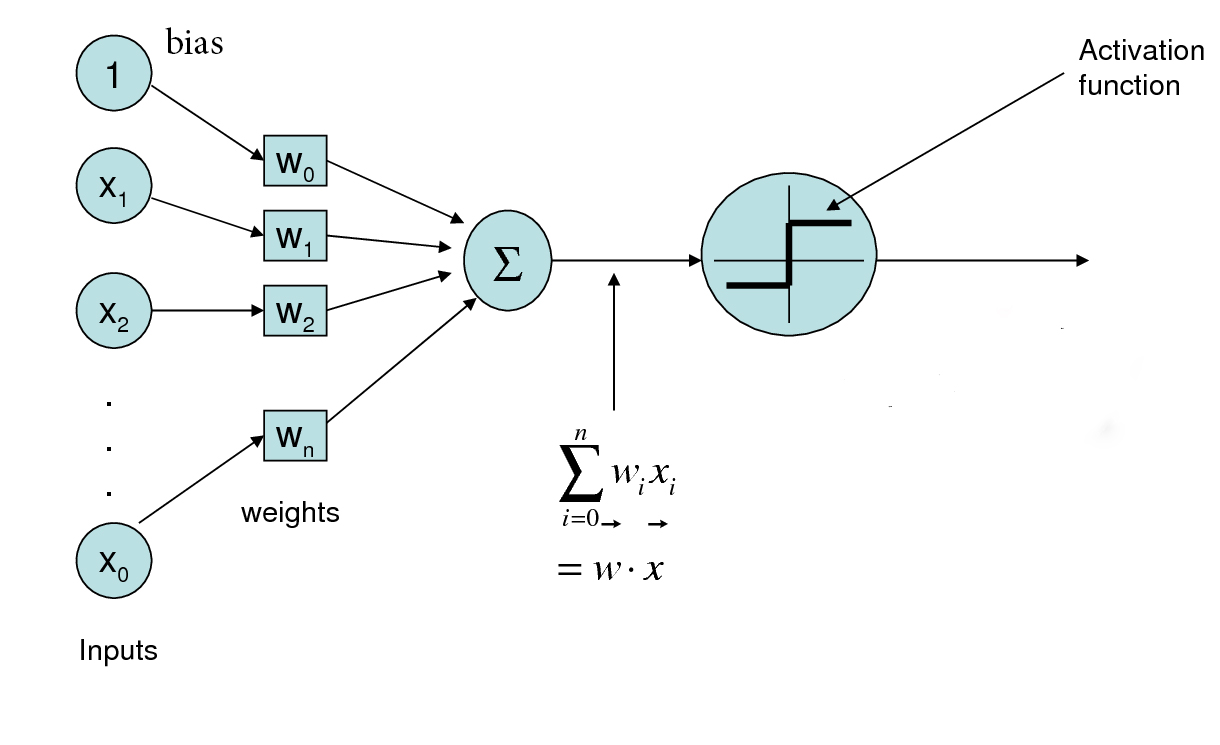
\includegraphics[width=14cm]{40-4}
	\caption{Perceptron}
	\label{odkaz}
	\centering
\end{figure}
\clearpage					      
Když máme tuto hodnotu\footnote{často bývá označována jako vnitřní potenciál}, tak použijeme aktivační funkci, které tuto hodnotu předáme jako parametr a výstup této funkce bude zároveň i výstupem perceptronu. To tedy znamená, že pokud si označíme $x_i$ jako $i$-tý prvek množiny vstupu, $w_i$ jako $i$-tý prvek množiny vah, $n$ jako velikost vstupu (stejná jako velikost pole vah), $\theta$ jako práh, $S$ jako aktivační funkci a $o$ jako výstup buňky, pak platí, že:

$$
	o~= S(\sum\limits_{i=0}^n w_ix_i + \theta)
$$
 \subsubsection{LSTM  buňka}
 Dalším typem neuronové buňky, která bude pro moji práci stěžejní, je buňka LSTM. Tato buňka obsahuje vždy pole vah, dále 3 brány\footnote{volně přeloženo z~anglického termínu gate} a hodnotu vnitřního stavu buňky. Na buňku je při každém jejím využití přivedeno pole vstupních hodnot, jehož délka je stejná jako délka pole vah a ta na základě hodnot v~branách a na vstupním poli upraví hodnotu ve svém vnitřním stavu a také vygeneruje výstup, který je dále předáván na zpracování jiným buňkám.\par
V~LSTM buňce nalezneme 3 typy bran, a to vstupní (input gate), výstupní (output gate) a bránu, která určí, kdy má buňka svůj stav zapomenout (forget gate). Tyto brány jsou v~buňce proto, aby rozhodly, jakou důležitost má vstup, výstup a vnitřní stav buňky a určují tím, jak moc je buňka ovlivněna hodnotami ze vstupu a naopak, jak ovlivňuje ostatní buňky svým výstupem. Tyto brány jsou reprezentovány reálným číslem, obvykle v~rozmezí mezi nulou a jedničkou s~tím, že čím je jejich hodnota nižší, tak tím je také menší důležitost věci, kterou mají na starost.\par
Další důležitou součástí sítě je pole vah. Toto pole je, jak jsem již zmínil, stejně velké, jako pole se vstupem a má takovou vlastnost, že každému prvku ze vstupu odpovídá právě jedna váha z~pole. Tyto váhy jsou reálná čísla, s~tím, že každá váha rozhoduje, jak moc je důležitá hodnota prvku vstupu, kterému daná váha odpovídá. Důležitost opět roste s~absolutní hodnotou váhy.\par
\begin{figure}[h]
	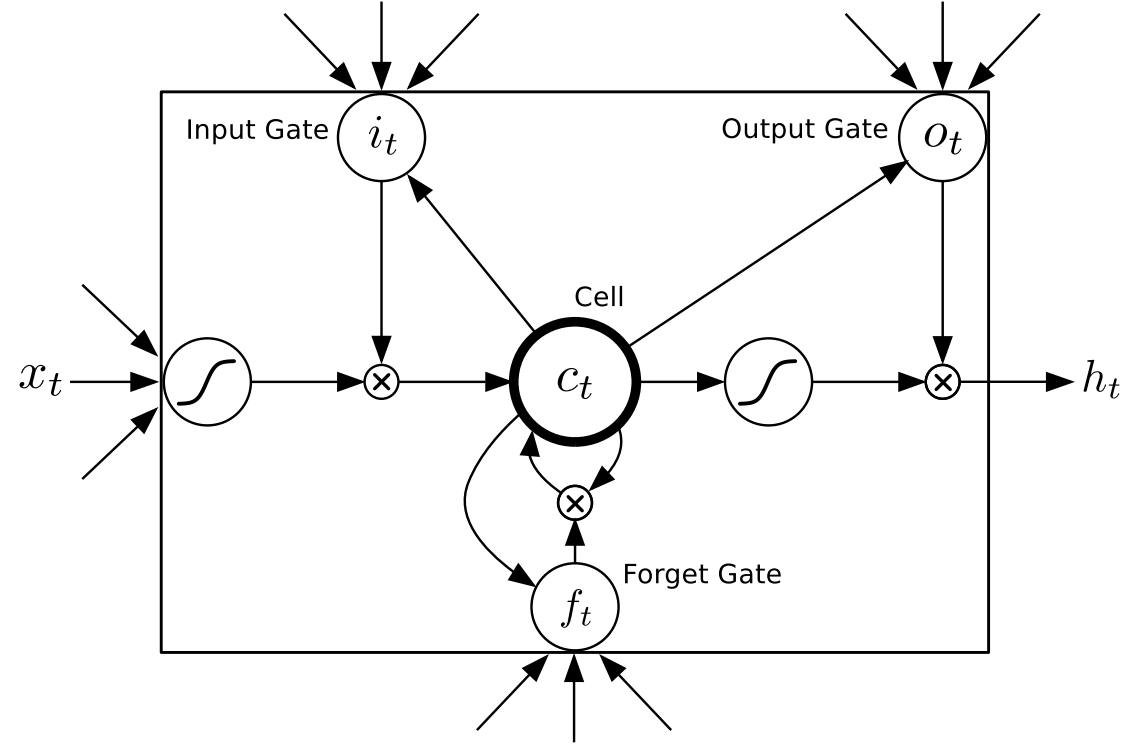
\includegraphics[width=14cm, height=8cm]{LSTM-cell.png}
	\caption{LSTM buňka}
	\label{odkaz}
	\centering
\end{figure}
\clearpage
Další částí buňky je vnitřní stav buňky. Jde o~hodnotu, vyjádřenou jako reálné nezáporné číslo, která vyjadřuje, co se s~buňkou dělo při jejích předchozích využitích.\par
Po předání vstupu buňce je počítána nejprve hodnota vstupu. Tato hodnota se vypočítá sečtením všech hodnot ve vstupu, s~tím, že každá hodnota má svoji důležitost, kterou do celkového výpočtu zakomponuji tak, že vynásobím každou hodnotu vstupu příslušnou vahou, tak výsledná hodnota vstupu bude odpovídat součtu těchto hodnot. Když si tedy vstupní hodnotu označíme jako $r$, dále si počet prvků na vstupu, tudíž i počet vah, označíme jako $n$, dále si prvek vstupu označíme jako $x_i$, kde $i$ bude pořadí, kolikátý se v~poli nachází a prvek v~poli vah si označíme jako $w_i$, kde $i$ bude pořadí, kolikátý prvek se v~poli vah $w$ nachází, tak vzorec pro výpočet vstupní hodnoty bude znít takto:$$r = \sum\limits_{i=0}^n w_ix_i$$
Tato hodnota je dále potřeba převést na vhodnou hodnotu mezi -1 a 1 pomocí aktivační funkce, které bude vypočítaná hodnota předána jako parametr. Nejčastěji se využívá funkce hyperbolický tangent, která splňuje všechny uvedené vlastnosti. Z~toho tedy vyplývá, že pokud zůstane označení proměnných stejné, pak bude hodnota vstupu rovna: $$r = \tanh(\sum\limits_{i=0}^n w_ix_i)$$\par
Nyní již projde vstup výpočtem a dostane se na input gate. Tato brána má rozhodnout, jak je tato vstupní hodnota důležitá. Jelikož je v~této bráně uloženo číslo mezi 0 a 1 s~tím, že čím je tato hodnota nižší, tím je méně důležitá, tak pokud touto hodnotou vstup vynásobíme, tak ho tím dostatečně upravíme dle důležitosti. To znamená, že vstup po projítí input gate bude při stejném označení proměnných za předpokladu, že input gate bude označena jako $g_i$, roven: $$r = g_i\cdot\tanh(\sum\limits_{i=0}^n w_ix_i)$$\par
Nyní již máme kompletně zjištěnou hodnotu vstupu v~buňce a můžeme pomocí ní upravit stav buňky. Ten upravíme tak, že ke stávajícímu stavu přičteme vstup, tudíž pokud vstup necháme jako $r$, a potom dále označíme $s$ stav buňky, který chceme získat a $s_0$ jako stav buňky, který byl v~buňce před jejím zavoláním, tak se stav vypočítá takto: $$s = s_0 + r$$což je po dosazení za $r$ ekvivalentní výrazu: $$s = s_0 + g_i\cdot\tanh(\sum\limits_{i=0}^n w_ix_i)$$.\par
Co se týče výstupu z~buňky, tak vrátíme hodnotu, kterou máme uloženou ve stavu buňky, s~tím rozdílem, že musíme vyhodnotit, jak moc je tento výstup důležitý. To zjistíme tak, že hodnotu ve stavu buňky vynásobíme hodnotou v~output gate a získáme tím hodnotu výstupu. Když si tedy výstup označíme jako $o$ a output gate jako $g_o$ a ostatní proměnné necháme jako dříve, tak musí platit: $$o = g_os$$ což je ekvivalentní s~výrazem: $$o = g_o(s_0 + g_i\cdot\tanh(\sum\limits_{i=0}^n w_ix_i))$$\par
Nyní je ještě potřeba vyhodnotit, zda je důležité si pamatovat dále stav či nikoliv. O~to se postará prozatím stále ještě nevyužitá forgery gate. Když hodnotou této brány vynásobíme hodnotou stavu buňky, tak hodnota zůstane nepozměněna pokud je důležitá (forgery gate je 1) a nebo klesne k~0, pokud důležitá není. To znamená, že pokud si forgery gate označíme jako $g_f$, tak finální stav buňky bude roven:$$s = g_f(s_0 + g_i\cdot\tanh(\sum\limits_{i = 0}^n w_ix_i))$$
Nyní shrňme 2 nejdůležitější vzorce této části a to jak vypočítat výstup a stav buňky ze vstupu za znalosti pole vah a bran:
\begin{align*}
	o~&= g_o(s_0 + g_i\cdot\tanh(\sum\limits_{i = 0}^n w_ix_i))\\
	s~&= g_f(s_0 + g_i\cdot\tanh(\sum\limits_{i = 0}^n w_ix_i))\\
\end{align*}
S~tím, že $o$ je výsledný výstup z~buňky, $s$ je výsledný stav buňky, $g_o$ je output gate, $g_f$ je forgery gate, $g_i$ je input gate, $s_0$ je původní stav buňky, $n$ je počet prvků na vstupu, $x_i$ představuje $i$-tý prvek vstupu a $w_i$ představuje váhu odpovídající $i$-tému prvku vstupu.
\par
\subsubsection{Výpočet hodnot na branách}
Jak je psáno v~předchozí kapitole, brány jsou hodnoty, které určují, jak je určitá informace důležitá. Hodnoty těchto bran závisí na dvou faktorech a to na vstupu, který daná buňka dostane a na buňce samotné. Je tomu tak, protože každá buňka musí reagovat jinak pokaždé, když dostane něco jiného (například pokud generuji text a dostanu, že před aktuálně generovaným znakem byla mezera, zapomenu předchozí slovo) a také každá buňka má na starosti jinou věc a tedy se 2 různé buňky musí zachovat jinak i když dostanou stejný vstup (když pro příklad opět využiji generování textu, tak buňka, která má na starosti oddělování slov zapomene svůj stav po každé mezeře, zatímco buňka na oddělování odstavců nikoliv). Dále v~rámci jedné buňky při stejném vstupu musí mít každá z~bran (jak input, tak output i forgery) jinou hodnotu, jelikož například je potřeba, aby buňka zapomněla svůj stav, ale její výstup bude velmi důležitý. To tedy musí nutně znamenat, že každá z~bran musí mít vlastní pole vah se stejnými vlastnostmi, jako má pole vah LSTM buňky popsané v~předešlé kapitole. Výsledná hodnota na váze se spočítá tak, že každý prvek ze vstupu vynásobíme odpovídající váhou z~pole vah patřícímu k~bráně, jejíž hodnotu počítám. To tedy znamená, že pokud si označíme $x_i$ jako $i$-tý prvek vstupu a $w_i$ jako $i$-tý prvek pole vah, dále $n$ jako počet prvků na vstupu a $g$ jako hodnotu váhy, kterou počítáme, tak dostaneme, že:$$g = \sum\limits_{i = 0}^n w_ix_i$$
Tuto hodnotu je také potřeba dále převést na hodnotu mezi nulou a jedničkou, jak je psáno v~předchozí kapitole. Na to použijeme funkci, jejíž obor hodnot je mezi nulou a jedničkou, které dříve vypočítaný výsledek předáme a výsledek této funkce bude již výsledná hodnota brány. K~tomuto se obvykle využívá funkce sigmoid. To tedy znamená, že při stejném označení proměnných se hodnota na bráně vypočítá jako:$$g = sig(\sum\limits_{i = 0}^n w_ix_i)$$
\subsubsection{Neuronová vrstva}
Neuronová vrstva je množina neuronových buněk stejného typu. Všechny tyto buňky mají všechna pole vah stejně velká. Každá vrstva při průchodu dat sítí dostane vstup ve tvaru pole čísel a má za úkol vygenerovat příslušný výstup. Při dodání vstupu vrstvě je toto pole předáno jako vstup všem buňkám ve vrstvě. To tedy znamená, že všechny buňky z~jedné vrstvy dostávají v~každém kroku stejný vstup. Každá buňka tento vstup zpracuje dle postupu popsaným v~předešlých kapitolách a vygeneruje jedno číslo, které je výstupem buňky. Dále se výstupy všech buněk vrstvy uloží do pole, které je samozřejmě dlouhé jako počet buněk ve vrstvě, a takto vzniklé pole hodnot je výstupem dané vrstvy.  
\subsubsection{LSTM síť}
LSTM síť je skupina neuronových vrstev, které bývají zpravidla typu LSTM, s~tím, že se zde mohou vyskytovat i vrstvy jiného typu. Tato síť obsahuje několik skrytých vrstev a jednu vrstvu výstupní\footnote{někdy se mluví také o~vrstvě vstupní, která však nemá žádný význam a se vstupem se nic nestane nebo je jako vstupní vrstva označována první vrstva skrytá}. Jako vstup bere síť pole hodnot stejně jako neuronová vrstva (viz kapitola dříve), která je v~síti umístěná jako první. Tento vstup daná vrstva zpracuje postupem popsaným v~předešlé kapitole a výstup je předán jako vstup další skryté vrstvě, která ho zpracuje a výstup opět předá dál. Poslední skrytá vrstva předá svůj výstup vrstvě výstupní a po jeho zpracování dostaneme výstup této vrstvy, který je zároveň výstupem sítě. Jak jsem již podotknul, tak LSTM síť nemusí obsahovat jen LSTM vrstvy, ale i vrstvy jiného typu. Obvykle je tomu tak, že skryté vrstvy typu LSTM bývají všechny, ale vrstva výstupní bývá v~některých případech typu jiného (samozřejmě může jí být i vrstva LSTM). V~mé práci jsem právě využil síť, která používá skryté vrstvy typu LSTM a vrstva výstupní je vrstva složená s~perceptronů, které bývá označována jako feed forward\footnote{zkráceně FF vrstva}.
\subsection{Učení LSTM sítí}
Tato kapitola se zabývá algoritmem, který slouží ke správnému nakonfigurování vah sítě, čímž naučíme síť tomu, aby generovala správné a očekávané výstupy. Nejprve v~této kapitole popíši, jak vypadají data, na kterých se síť učí a následně algoritmus Back Propagation, který slouží k~učení dopředných sítí a jeho úpravu pro učení sítí rekurentních.
\subsubsection{Formát trénovacích dat}
Jako vstupní data pro funkci, která slouží k~učení sítí bude datová řada, což bude uspořádaná množina několika uspořádaných dvojic formátu vstup a předpokládaný výstup. Tyto řady jsou seskupeny do takzvaného datasetu, přičemž jde o~neuspořádanou množinu, tudíž nezáleží na tom, v~jakém pořadí jsou samotné řady dat zpracovávány (což se o~prvcích, které jsou v~řadě, říci nedá).\par
Představme si jako příklad síť, která slouží ke generování textu. Zde může být dataset nějaký delší text, článek nebo kniha, která je dělena do odstavců. Jako řada dat bude jeden odstavec textu, jejíž prvky budou jednotlivá písmena, s~tím, že ke každému písmenu bude jako předpokládaný výstup písmeno následující.
\subsubsection{Back Propagation}
Back Propagation je algoritmus, který slouží k~učení většiny dopředných neuronových sítí. Pro jeden svůj krok jako vstup přijímá uspořádanou dvojici vstupu a předpokládaného výstupu, přičemž pokaždé upraví váhy a opakuje se na jiné dvojici dat. Následně se daný vstup předá jako vstup sítě a síť vygeneruje svůj výstup, který se porovná s~výstupem předpokládaným a vypočítám tím odchylku sítě. Je jasné, že pro každou konfiguraci sítě bude i jiný výstup sítě a tudíž i jiná chyba sítě. To tedy znamená, že lze vytvořit funkci chyby sítě v~závislosti na různých konfiguracích sítě, tedy funkci $J: \mathbb{R}^n \rightarrow \mathbb{R}$, kde $\mathbb{R}^n$ je prostor hodnot všech parametrů. Naším úkolem je najít takovou konfiguraci sítě, pro kterou je chyba co nejnižší, tudíž najít globální minimum\footnote{Jde o~ideální případ, ovšem v~praxi je tuto konfiguraci nemožné najít a tudíž se snažíme funkci co nejvíce minimalizovat obvykle nalezením lokálního minima} chybové funkce, k~čemuž využijeme takzvané gradientní metody. Ta je založena na tom, že pro každý bod funkce jsme schopni pomocí výpočtů určit směr\footnote{Obvykle bývá označován jako gradient}, ve kterém chyba sítě klesá nejrychleji. Následně aktualizujeme aktuální konfiguraci sítě v~tomto směru.\par
Pro tento algoritmus je také velmi důležitý parametr zvaný learning rate, který udává, jak daleko ve směru gradientu pro jednu dvojici vstupu a výstupu půjdeme. Čím je tato hodnota vyšší, tím rychleji se pochopitelně síť učí, avšak na úkor přesnosti. Pokud tedy chceme mít síť naučenou rychle, volíme obvykle hodnotu tohoto parametru co nejvyšší a pokud chceme naopak velmi přesně síť naučit, nastavujeme tuto hodnotu velmi nízko. My však chceme najít kompromis mezi těmito extrémy a to naučit síť přiměřeně rychle, ale také uspokojivě dobře. K~tomu se obvykle používá technika, která funguje tak, že z~počátku volíme learning rate poměrně vysoko a postupně jej snižujeme, čímž docílíme toho, že zpočátku, když síť nic neumí se učí poměrně rychle a až se dostaneme ke konfiguraci, která generuje náznaky výsledků, tak je již learning rate poměrně nízký a síť se tak již postupně zdokonaluje a zpřesňuje své výsledky ke správnému naučení.\par
\begin{figure}[h]
	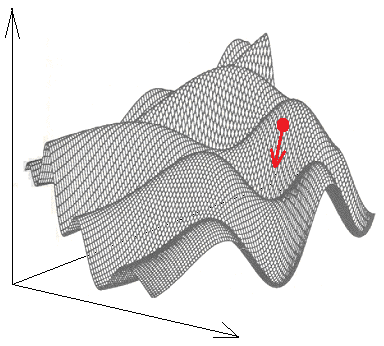
\includegraphics[width=14cm]{backpropagation.png}
	\caption{Ukázka funkce $J$ pro 2 parametry sítě}
	\label{odkaz}
	\centering
\end{figure}
\clearpage
Když algoritmus shrnu do pseudokódu\footnote{parafrázováno ze zdroje: https://www.root.cz/clanky/biologicke-algoritmy-5-neuronove-site/, 20.1.2017}, mohl by vypadat nějak takto:
\begin{enumerate}
	\item Předej síti vstup, který funkce dostala a vygeneruj z~ní výstup
	\item Vypočítej chybu sítě
	\item Na základě vzorců uvedených níže vypočítej nové hodnoty vah a nahraj je místo hodnot původních
	\item Sniž learning rate
	\item Opakuj pro novou dvojici vstupu a výstupu 
\end{enumerate} \par
Nyní už jen chybí uvést, jak vypočítat nové hodnoty na vahách. Odvození a vysvětlení vzorců vyžaduje znalost pokročilé matematiky a není pro implementaci algoritmu stěžejní, proto se jím zde nebudu zabývat\footnote{pokud vás zajímá, kde se tyto vzorce vzali, zkuste se podívat například do knihy Teoretické otázky neuronových sítí, kterou přeložil Jiří Šíma s~Janem Nerudou na stranách 53-61}. Když si tedy označíme vstupy sítě jako $x_0 - x_n$, očekávaný výstup jako $o_0 - o_n$, dále když $y^n_i$ bude výstup $i$. neuronu $n$. vrstvy, $w^n_{ij}$ bude váha mezi $i$. neuronem $n-1$. vrstvy a $j$. neuronem $n$. vrstvy, $E^n_i$ bude chyba $i$. neuronu $n$. vrstvy a $L$ bude learning rate sítě a značená $A \leftarrow B$ bude značit, že do proměnné $A$ nahrajeme proměnnou $B$, pak budou váhy přepočítány následovně:
\begin{align*}
	E^{n}_j &= y^{n}_j(1-y^{n}_j)(o_j - y^{n}_j)\\\
	\Delta w^{n}_{ij} &= LE^{n}_jy_i^{(n-1)}~\footnotemark\\
	w^n_{ij} &\leftarrow w^n_{ij} + \Delta w^n_{ij}
\end{align*}
\footnotetext{pokud je $n - 1 = 0$, použije se $x_i$}
\subsubsection{Back Propagation through time}
Back Propagation through time je algoritmus, který slouží k~učení rekurentních neuronových sítí, tudíž i sítí LSTM, který ve své práci používám. Ve své podstatě funguje podobně jako klasický Back Propagation s~tím rozdílem, že je pouštěn na uspořádanou množinu testovacích vzorů a v~rámci této trénovací řady si uchovává svůj vnitřní stav. Když tento algoritmus shrnu do pseudokódu\footnote{parafrázováno ze zdroje: https://en.wikipedia.org/wiki/Backpropagation\_through\_time, 19-1-2017}, mohl by vypadat přibližně takto:
\begin{enumerate}
	\item Vynuluj vnitřní stav sítě (hodnoty, které si buňky pamatují)
	\item Proveď pro všechny prvky (uspořádaná dvojice ($input$,$output$)) v~trénovací řadě:
		\begin{enumerate}
			\item Spusť síť se vstupem v~prvku $input$ a vygeneruj výstup
			\item Vypočítej chybu sítě jako rozdíl vygenerovaného výstupu a předpokládaného výstupu v~proměnné $output$
			\item Tuto chybu zpět šiř pomocí algoritmu Back Propagation, spočítej nové hodnoty na vahách a váhy aktualizuj			
		\end{enumerate}
	\item Celé opakuj pro další řadu dat
\end{enumerate}
\begin{center}
\clearpage
\section{Vlastní LSTM Síť}
\end{center}
V~této kapitole popíši LSTM síť, kterou jsem vytvořil a použil ji ke generování textu. Tuto síť jsem psal v~jazyce C\# a kromě knihoven rozhraní .Net Framework jsem ještě využil knihovnu Sharp-ML-Recurent\footnote{Ke stažení na adrese: https://github.com/andrewfry/SharpML-Recurrent}, kterou jsem však musel patřičně upravit. Pro fungování programu je potřeba verze .Net Framework 3.6 nebo vyšší.
\subsection{Sturktura sítě}
Moje síť obsahuje 2 skryté vrstvy typu LSTM a jednu vrstvu výstupní typu Feed Forward. Dále by se dalo hovořit ještě o~vrstvě vstupní, která však se vstupem nic nedělá, jen předá celý vstup každému z~neuronů 1. skryté vrstvy. Obě skryté vrstvy obsahují 128 neuronů a jelikož jde o~síť klasifikační, tak velikost výstupní vrstvy je rovna počtu různých znaků, které se vyskytují v~trénovacím souboru, stejně tak jako velikost vstupu. V~případě mého tréninkového souboru jich bylo 39. Jako vstup dostává síť písmeno a má za úkol vygenerovat písmeno následující. Avšak jelikož síť nemůže pracovat se znaky, tak vstupní písmeno reprezentuji jako pole o~velikosti stejném jako pole znaků s~tím, že každému znaku odpovídá jeden prvek v~poli a tak jako vstup dostane síť pole, kde prvek, kterému odpovídá vstupní písmeno pole bude mít hodnotu jedna a ostatní prvky hodnotu 0. Síť pak vygeneruje pole, které funguje stejně jako pole vstupní, s~tím, že jelikož jsem jako aktivační funkci sítě zvolil sigmoid, tak každý prvek bude obsahovat číslo od 0 do 1 s~tím, že čím je tato hodnota vyšší, tím je větší pravděpodobnost, že tomuto poli odpovídající znak bude následujícím písmenem.
\subsection{Softmaxová vrstva}
Aby šlo o~pravděpodobnost v~pravém slova smyslu a aby se s~ní dobře pracovalo, pak součet všech prvků v~poli musí být roven jedné, což však většinou u~výstupu sítě nebývá. To znamená, že potřebujeme upravit hodnoty výstupu sítě tak, aby jejich součet byl roven 1 a zároveň, aby se nezrušil poměr mezi jednotlivými prvky a k~tomu se využívá právě technika softmaxové vrstvy. Nyní aplikujeme na data softmaxovou vrstvu. Ta funguje tak, že každý prvek v~poli vydělíme součtem všech prvků v~poli. Po tomto upravení nám jistě zůstane poměr mezi všemi prvky stejný, jelikož pokud vydělíme čitatele i jmenovatele zlomku stejným číslem, tak se poměr nezmění:
$$
	\frac{a}{b} = \frac{ac}{bc} = \frac{\frac{a}{c}}{\frac{b}{c}}
$$
Dále součet všech prvků musí být jedna, jelikož, za předpokladu že $A$ je původní množina prvků, platí, že:
$$
	\sum\limits_{a \in A}^{}\frac{a}{\sum\limits_{b \in A}^{}b} = \frac{\sum\limits_{a \in A}^{}a}{\sum\limits_{b \in A}^{}b} = 1
$$
\begin{lstlisting}[language=C, title={Ukázka kódu softmaxové vrstvy (i s~převodem na nezáporná čísla)}]

public static double[] Softmax(double[] field)
{
	double[] result = new double[field.Length];
	double sum = field.Sum();
	for(int i =  0; i < result.Length; i++)
	{
		result[i] = field[i] / sum;
	}
	return result;
}
\end{lstlisting}
\subsection{Výběr výsledného znaku}
Nyní již máme pole, které síť vygenerovala, převedena na čísla mezi 0 a 1, jejichž součet je roven 1 a potřebujeme z~něho jen vybrat ten správný prvek. Hned na první pohled se nabízí, že by se mělo vybrat maximum sítě, avšak pokud bychom zvolili tuto možnost, síť by se dříve či později zacyklila a opakovala by stále to samé. Ve spoustě případů totiž přichází v~úvahu více než jedno písmeno. Když si například vezmeme, že síť zatím vygenerovala písmena ca, tak dalším písmenem může být klidně t jako cat, nebo r jako car nebo m jako camera případně n jako can a spousta dalších a naopak písmena, jako je například a nebo x v~úvahu vůbec nepřicházejí. To tedy znamená, že pokud je síť správně naučená, tak by tato zmíněná a ještě další písmena, která přichází v~úvahu měla mít prav\-dě\-po\-dob\-nost všechna obdobně vysokou a písmena, která v~úvahu nepřipadají naopak pravděpodobnost velmi nízkou. To tedy znamená, že potřebujeme náhodně vybrat libovolné písmeno s~uspokojivě vysokou pravděpodobností. K~tomu se dá využít technika, která si na začátku zvolí proměnnou, která je rovna 1, nazvěme ji $mass$ a dále postupně prochází pole s~pravděpodobnostmi písmen a pro každý prvek udělá to, že porovná náhodně vygenerované číslo mezi 0 a 1 s~hodnotou podílu tohoto prvku a proměnné $mass$ a pokud je tento podíl větší, pak vrátí právě tento prvek a pokud ne, tak odečte od hodnoty proměnné $mass$ hodnotu aktuálně zkoumaného prvku a přesune se na další prvek.\par
Nejprve dokažme, že tato technika vždy vybere nějaký prvek. Předpokládejme, že tato technika zatím nevybrala žádný prvek a zrovna běží na posledním. V~tomto případě, jelikož proměnná $mass$ byla původně 1 a poté se od ní odečítaly vždy hodnoty ostatních prvků, tak bude v~proměnné $mass$ hodnota, která je rovna 1 - součet všech čísel v~poli, krom posledního a jelikož součet všech čísel v~poli je 1, tak pokud zvolím $a$ jako hodnotu posledního prvku, bude $mass = 1 - (1 - a) = a$. Jelikož porovnávám s~náhodně vygenerovaným číslem hodnotu podílu $a$ a $mass$, tak je jasné, že $\frac{a}{mass} = \frac{a}{a} = 1$, což je vždy větší než číslo mezi 0 a 1, tudíž je jasné, že pokud se hledání dostane až k~poslednímu prvku, tak jej vybere, tudíž tato technika vždy vybere nějaký prvek.\par
Nyní je ještě potřeba ukázat, že tato technika vybírá číslo, které má relativně vysokou prav\-dě\-po\-dob\-nost. Pokud je síť správně naučená, tak by měla generovat čísla, která nepřichází v~úvahu velice nízko, obvykle s~pravděpodobností do 1 \%. To tedy znamená, že podíl této hodnoty s~proměnnou $mass$ bude také velice nízký a tak je opravdu minimální pravděpodobnost, že by náhodně vygenerované číslo, se kterým tuto hodnotu porovnávám bylo menší než tento podíl. Naopak pokud bude znak v~úvahu přicházet, tak bude podíl s~proměnnou $mass$ relativně vysoký a tak tedy je poměrně vysoká pravděpodobnost, že náhodné číslo bude menší než hodnota podílu. Dělení hodnotou $mass$ je zde z~toho důvodu, že pokud bude v~úvahu přicházet hodně písmen, pravděpodobnost se mezi ně přibližně rovnoměrně rozmístí a tak nebude až tak příliš vysoká, jako když je takových písmen málo, ale stále výrazně vyšší, než pravděpodobnost písmen, která v~úvahu vůbec nepřicházejí. To tedy znamená, že potřebujeme jejich hodnotu postupně zvyšovat, aby jsme mohli výsledek vůbec vybrat, což nám umožňuje právě proměnná $mass$.
\begin{lstlisting}[language=C, title={Ukázka kódu pro výběr prvku z~pole}])

public static int FindIndex(Random rnd, double[] field)
{
	double mass = 1.0;
	for(int i = 0; i < field.Length; i++)
	{
		if(rnd.NextDouble() < field[i] / mass) return i;
		mass -= field[i];
	}
	return 0; //K tomuto nikdy nedojde, je to tu jen pro kompilaci
}
\end{lstlisting}
\subsection{Třídy Matrix a Graph a rozhraní ILayer a INonlinearity}
V~této části popíši třídy, které jsou potřebné k~reprezentaci sítě a její jednotlivých vrstev. První takovou třídou je třída Matrix, která reprezentuje matici, kde bývají obvykle uloženy váhy sítě nebo se také používá jako vstup či výstup vrstvy a v~obdobných situacích. Tato třída obsahuje pět proměnných a to proměnné $Rows$, $Cols$ typu int, které určují rozměry matice a dále 3 matice typu bool[] a to matice $W$, $Dw$ a $StepCache$. Matice je v~poli reprezentována tak, že prvek $x_{ij}$ najdeme jako např. $W[i*j + i]$. Dále tato třída obsahuje 3 konstruktory, z~nichž jeden umožní nastavit všechny parametry, další jen pole $W$ a další jen proměnné $Rows$ a $Cols$. Dále obsahuje funkci Clone, která matici zkopíruje do jiné, funkce resetDw a resetStepCache, které vynulují hodnoty v~příslušných polích, funkci transpose, která matici přepíše tak, že prohodí její rozměry, ale pořadí prvků zachová, funkci Random, která nastaví prvky v~proměnné $W$ na náhodná čísla mezi 0 a 1, dále funkci Ident, která vytvoří čtvercovou matici s~hodnotami 1 na uhlopříčce a 0 na zbytku a nakonec funkci Uniform, která vytvoří matici o~zadaných rozměrech a která bude mít všechny prvky v~proměnné $W$ nastaveny na hodnotu, kterou dostane v~parametru. Tato třída obsahuje ještě další veřejné funkce, ale ty již nejsou pro nás zas tak příliš podstatné nebo jsou jen voláním jiných funkcí s~některým fixním parametrem.\par
Dále budeme potřebovat třídu Graph, která obsahuje metody pro početní operace s~maticemi. Tato třída obsahuje dvě proměnné, jednu logickou, která určuje, zda se nacházíme v~učícím procesu či nikoliv, a další je seznam rozhraní IRunnable, která je však použita pouze při učení sítě a tím se nyní nebudu zabývat. Dále tato třída obsahuje funkci ContactVectors, která spojí 2 matice s~výškou 1 do matice jedné, funkci NonLin, která vynuluje proměnné $Dw$ a $Stepcache$ matice a na všechny prvky pole $W$ aplikuje nelineární funkci, poté funkci Mul, která mezi sebou vynásobí 2 matice, funkci Add, která 2 matice sečte, funkci Substract, která od sebe 2 matice odečte a funkci Elmul, která vynásobí odpovídající si prvky 2 matic. Opět i tato třída obsahuje další veřejné funkce, avšak mimo proces učení pro nás nejsou nijak zajímavé a nebo jde o~volání jiných funkcí s~konkrétním parametrem.\par
Dále je v~reprezentaci sítě využito rozhraní INonlinearity, ze kterého dědí všechny aktivační funkce a to konkrétně funkce lineární, rektifikovaná lineární\footnote{funkce, která se chová takto: $f(x \ge 0) = x \wedge f(x < 0) = 0$}, sinus, sigmoid a hyperbolický tangent. Toto rozhraní obsahuje 2 funkce a to funkci Forward, která vrátí funkční hodnotu dané funkce v~určitém bodě a dále funkci Backward, která vrátí funkční hodnotu zderivované funkce v~určitém bodě.\par
Poslední je rozhraní ILayer, ze kterého dědí všechny typy neuronových vrstev. Toto rozhraní obsahuje 3 funkce a to funkci Activate, která dá vrstvě určitý vstup a tato vrstva následně vygeneruje výstup, dále funkci ResetState, která v~případě, že mají buňky v~síti nějaký vnitřní stav, tak jej vynuluje a nakonec funkci GetParameters, která vrátí seznam matic, který bude obsahovat všechny matice, které se v~síti nachází.
\begin{lstlisting}[language=C, title={Ukázka rozhraní INonlinearity a ILayer}]

public interface INonlinearity
{
	double Forward(double x);
	double Backward(double x);
}
public interface ILayer
{
	Matrix Activate(Matrix input, Graph g);
	void ResetState();
	List<Matrix> GetParameters();
}
\end{lstlisting}
Třídy Matrix a Graph jsou příliš dlouhé, proto sem nebudu jejich kód celý uvádět, jen pro ukázku zde uvedu 1 funkci z~každé z~těchto tříd.
\begin{lstlisting}[language=C, title={Ukázka funkce Ident ze třídy Matrix a funkce Add ze třídy Graph}]

public static Matrix Indent(int dim)
{
	Matrix result = new Matrix(dim, dim);
	for(int i = 0; i < dim; i++)
	{
		result.setW(i, i, 1.0);
	}
	return result;
}
public Matrix Add(Matrix m1, Matrix m2)
{
	if(m1.Rows != m2.Rows || m1.Cols != m2.Cols)
	{
		throw new Exception("Matrix dimension mismatch";)
	}
	Matrix returnObj = new Matrix(m1.Rows, m1.Cols);
        for (int i = 0; i < m1.W.Length; i++)
        {
            returnObj.W[i] = m1.W[i] + m2.W[i];
        }
        if (this.ApplyBackprop) //pouze pokud jsem v~rezimu uceni site
        {
            Runnable bp = new Runnable();
            bp.Run = delegate()
            {
                for (int i = 0; i < m1.W.Length; i++)
                {
                    m1.Dw[i] += returnObj.Dw[i];
                    m2.Dw[i] += returnObj.Dw[i];
                }
            };
            Backprop.Add(bp);
    }
        return returnObj;

}
\end{lstlisting}
\subsection{Reprezentace Feed Forward vrstvy}
Jak jsem již psal, perceptron, ze kterých se skládá tato vrstva si musí pamatovat 3 věci, pole vah, bias a druh aktivační funkce, která je však pro všechny buňky v~1 vrstvě stejná. To tedy znamená, že FF vrstva si musí pamatovat matici vah ve formátu, že každý řádek matice odpovídá jednomu neuronu, dále matici biasů, která má jen jeden řádek a každý prvek tohoto řádku odpovídá určitému neuronu a nakonec si musí pamatovat typ aktivační funkce, která bude použita. Třída, která reprezentuje FF vrstvu tedy obsahuje 2 proměnné typu Matrix a to proměnné $\_w$, která reprezentuje matici vah a $\_b$, která reprezentuje matici biasů. Dále obsahuje proměnnou typu INonlinearity s~názvem $\_f$, která obsahuje příslušnou aktivační funkci. Dále, jelikož jako každá neuronová vrstva i FF vrstva dědí z~rozhraní ILayer, tak musí obsahovat funkce Activate, ResetState a GetParameters. Funkce Activate vypočítá na základě vstupu vrstvy i její výstup stejným principem, který je popsán v~sekci 2.1.1. Jelikož vrstva neobsahuje žádný svůj vnitřní stav, tak není třeba vnitřní stav vrstvy nulovat, tudíž funkce ResetState neudělá vůbec nic. Následuje funkce GetParameters, která vrátí list instancí třídy Matrix, a to konkrétně matice $\_w$ a $\_b$, v~tomto pořadí. Nakonec je třeba dodat, že třída obsahuje také 2 konstruktory, z~nichž jeden z~nich přijímá rovnou matice $\_w$, $\_b$ a aktivační funkci, které nastaví za proměnné a druhý přijímá počet vstupů, počet neuronů ve vrstvě, typ aktivační funkce, parametr, který určí, jak daleko od průměru budou náhodně vygenerované váhy a instanci třídy Random a následně tuto vrstvu nově vygeneruje s~náhodně nastavenými vahami.
\begin{lstlisting}[language=C, title={Ukázka třídy FeedForwardLayer}]

public class FeedForwardLayer : ILayer
{
        public readonly Matrix _w;
        public readonly Matrix _b;
        public readonly INonlinearity _f;

	//konstruktory vrstvy, nebylo je nutne uvadet

        public Matrix Activate(Matrix input, Graph g)
        {
            Matrix sum = g.Add(g.Mul(_w, input), _b);
            Matrix returnObj = g.Nonlin(_f, sum);
            return returnObj;
        }

        public void ResetState()
        {

        }

        public List<Matrix> GetParameters()
        {
            List<Matrix> result = new List<Matrix>();
            result.Add(_w);
            result.Add(_b);
            return result;
	}
    }

\end{lstlisting}
\subsection{Reprezentace LSTM vrstvy}
Pro LSTM síť je nejzásadnější LSTM vrstva o~jejíž reprezentaci se stará právě třída LstmLayer. Tato vrstva je složena z~buněk LSTM, které si musí pamatovat poněkud více věcí než perceptron. Každá buňka si totiž musí pamatovat stejně jako perceptron svůj bias a pole vah, avšak krom toho je ještě potřeba si pamatovat vnitřní stav této buňky a také pole vah a bias pro každou z~bran buňky. To tedy znamená, že pro reprezentaci LSTM vrstvy si potřebujeme pamatovat vnitřní stavy všech buněk, o~což se postará třída Matrix ve formátu matice o~jednom řádku s~počtem sloupečků stejným jako je dimenze vrstvy s~tím, že hodnota v~každém sloupci odpovídá danému neuronu. Stejným způsobem budou reprezentovány i biasy buněk a to jak jejich biasy vstupní tak biasy na jejich branách. Váhy vrstvy budou opět reprezentovány jako matice, tudíž instance třídy Matrix, které budou ve formátu, že každý řádek bude odpovídat určitému neuronu a bude obsahovat celé pole vah. Takto opět reprezentujeme nejen váhy buňky, ale také váhy u~každé z~bran. Dále si musíme pamatovat ještě 2 hodnoty a to jsou velikost vstupu, která odpovídá velikosti předchozí vrstvy a dále velikost výstupu, která je stejná jako počet neuronů ve vrstvě. Nakonec si ještě musíme uložit typy aktivačních funkcí, které jsou však vždy v~případě bran funkce Sigmoid a v~případě buňky samotné hyperbolický tangent\par
Jelikož i tato třída, stejně jako všechny ostatní vrstvy, dědí z~rozhraní ILayer, musí obsahovat metody Activate, která vrstvě předá vstup a vygeneruje výstup způsobem popsaným v~teoretické části práce, dále funkci ResetState, která vynuluje matici s~vnitřním stavem buňky a nakonec funkci GetParameters, která vrátí seznam všech matic, které se ve vrstvě vyskytují.\par
Ještě je potřeba dodat, že vrstva obsahuje 2 konstruktory, kde jeden z~nich dovoluje zadat všechny proměnné, které následně nastaví a ten druhý dostane pouze hodnoty vstupní a výstupní dimenze, instanci třídy Random a hodnotu, která určí rozsah hodnot vah a všechny váhy i biasy vygeneruje náhodně.
\begin{lstlisting}[language=c, title={Ukázka třídy LstmLayer}]

public class LstmLayer : ILayer
{
    public int _inputDimension;
    public readonly int _outputDimension;

    public readonly Matrix _wi;
    public readonly Matrix _inputBias;
    public readonly Matrix _wf;
    public readonly Matrix _	forgetBias;
    public readonly Matrix _wo;
    public readonly Matrix _outputBias;
    public readonly Matrix _wc;
    public readonly Matrix _cellWriteBias;

    public Matrix _cellContext;

    public readonly INonlinearity _inputGateActivation = new SigmoidUnit();
    public readonly INonlinearity _forgetGateActivation = new SigmoidUnit();
    public readonly INonlinearity _outputGateActivation = new SigmoidUnit();
    public readonly INonlinearity _cellInputActivation = new TanhUnit();
    public readonly INonlinearity _cellOutputActivation = new TanhUnit();


    //konstruktory vrstvy
    
    public Matrix Activate(Matrix input, Graph g)
    {
	    //telo tridy Activate
    }

    public void ResetState()
    {
        _cellContext = new Matrix(_outputDimension);
    }

    public List<Matrix> GetParameters()
    {
        List<Matrix> result = new List<Matrix>();
        result.Add(_wi);
        result.Add(_inputBias);
        result.Add(_wf);
        result.Add(_forgetBias);
        result.Add(_wo);
        result.Add(_outputBias);
        result.Add(_wc);
        result.Add(_cellWriteBias);
        return result;
    }
}


\end{lstlisting}
\subsection{Reprezentace neuronové sítě}
O~reprezentaci neuronové sítě se stará třída NeuralNetwork, která dědí z~rozhraní INetwork, které vypadá úplně stejně, jako rozhraní ILayer. Jelikož neuronová síť je vlastně množina neuronových vrstev, tak jediné, co si u~ní musíme pamatovat jsou vrstvy, které obsahuje. Jelikož všechny  vrstvy dědí z~rozhraní ILayer, tak se nabízí jako nejjednodušší způsob, jak si tyto vrstvy zapamatovat, seznam rozhraní ILayer. To tedy znamená, že třída NeuralNetwork obsahuje jen jedinou proměnnou a to proměnnou $\_layers$ typu List$<$ILayer$>$. Dále obsahuje jeden konstruktor, který přijímá jako parametr právě seznam vrstev a nahraje jej do proměnné $\_layers$. Dále, jelikož dědí z~rozhraní INetwork, které je stejné jako ILayer, tak musí obsahovat funkce Activate, ResetState a GetParameters. Funkce Activate má za úkol ze zadaného vstupu sítě vygenerovat výstup, tudíž projíždí postupně všechny vrstvy a volá na nich jejich funkci Activate, s~tím, že jako vstup vrstvy předá výstup  vrstvy předchozí a samozřejmě vrátí výstup poslední vrstvy jako výstup sítě. Funkce ResetState zavolá funkci ResetState všech svých vrstev a tím vynuluje vnitřní stav celé sítě a nakonec funkce GetParameters postupně zavolá funkci GetParameters na všech svých vrstvách a jejich výsledky spojí a vrátí.
\begin{lstlisting}[language=C, title={Ukázka třídy NeuralNetwork}]

public class NeuralNetwork : INetwork
{  
    public readonly List<ILayer> _layers;

    public NeuralNetwork(List<ILayer> layers)
    {
        this._layers = layers;
    }

    public Matrix Activate(Matrix input, Graph g)
    {
        Matrix prev = input;
        foreach (ILayer layer in _layers)
        {
            prev = layer.Activate(prev, g);
        }
        return prev;
    }

    public void ResetState()
    {
        foreach (ILayer layer in _layers)
        {
            layer.ResetState();
        }
    }

    public List<Matrix> GetParameters()
    {
        List<Matrix> result = new List<Matrix>();
        foreach (ILayer layer in _layers)
        {
            result.AddRange(layer.GetParameters());
        }
        return result;
    }
}
\end{lstlisting}
\subsection{Třída NetworkBuilder}
Třída NetworkBuilder, jak již název napovídá, má za úkol vybudovat ze zadaných parametrů novou síť. Tato třída obsahuje metody MakeLstm, MakeLstmWithInputBottleneck, MakeFeedForward, MakeGru a Make Rnn, které vytvoří příslušný typ sítě. Nás však ostatní typy sítě příliš nezajímají a tak popíši pouze funkci MakeLstm. Tato funkce dostane jako vstup parametry, které udávají velikost vstupu, výstupu a skrytých vrstev, dále počet skrytých vrstev, typ aktivační funkce, která bude použita jako aktivační funkce výstupní vrstvy, hodnotu, která určí rozsah náhodně vygenerovaných vah a nakonec instanci třídy Random. Jako výstup vrátí tato metoda síť, kterou na základě těchto parametrů vytvořila.

\begin{lstlisting}[language=C, title={Ukázka funkce MakeLstm}]
public static NeuralNetwork MakeLstm(int inputDimension, int hiddenDimension, int hiddenLayers, int outputDimension, INonlinearity decoderUnit, double initParamsStdDev, Random rng)
{
	List<ILayer> layers = new List<ILayer>();
        for (int h = 0; h < hiddenLayers; h++)
        {
            if (h == 0)
            {
                layers.Add(new LstmLayer(inputDimension, hiddenDimension, initParamsStdDev, rng));
            }
            else
            {
                layers.Add(new LstmLayer(hiddenDimension, hiddenDimension, initParamsStdDev, rng));
            }
        }
        layers.Add(new FeedForwardLayer(hiddenDimension, outputDimension, decoderUnit, initParamsStdDev, rng));
        return new NeuralNetwork(layers);
}
\end{lstlisting}
Ještě je potřeba poznamenat, že tato třída obsahuje také metody pro načítání a ukládání sítě, které popíši v~následující kapitole.
\subsection{Ukládání sítě}
Jelikož je nesmysl síť po každém spuštění znovu učit, tak je potřeba si pamatovat její stav. Pro uložení sítě jsem zvolil formát adresářové struktury. Celá síť je uložená ve složce LSTMNetwork. Tato složka obsahuje 3 prvky a to soubor info.csv, kde je napsáno, kolik síť obsahuje skrytých vrstev a 2 podsložky hidden a output, které obsahují skryté a výstupní vrstvy sítě. Každá vrstva je opět reprezentována složkou, která obsahuje soubor info.csv a poté všechny matice, které daná vrstva obsahuje, s~tím, že každá matice je v~odděleném souboru opět ve formátu csv, který nese stejný název jako proměnná, které tato matice odpovídá. Soubor info.csv obsahuje všechny informace, které vrstva potřebuje a které nejsou uloženy v~maticích. V~případě FF vrstvy jde o~typ aktivační funkce sítě a v~případě vrstvy LSTM jde o~velikost vstupní a výstupní vrstvy.\par
O~ukládání a zpětné načítání sítě se starají funkce LoadLSTM a SaveLSTM, které se nacházejí ve třídě NetworkBuilder.
\clearpage
\begin{center}
\section{Učení vlastní sítě}
\end{center}
\subsection{Třídy DataSet, DataSequence, DataStep, FieldLetterTranslator a DataTextGenerator a rozhraní ILoss}
Nejprve, než začneme probírat učení samotné, musíme si představit několik tříd a rozhraní, které nám slouží pro reprezentaci trénovacích dat a jako nástroje pro učící algoritmus. Třídy DataSet, DataSequence a DataStep jsou třídy sloužící k~reprezentaci trénovacích dat. Jak jsem psal dříve, Back Propagation through time potřebuje data ve formátu množina uspořádaných množin uspořádaných dvojic. Třída DataStep reprezentuje tu nejmenší částečku dat a to dvojici vstup a předpokládaný výstup. To tedy znamená, že tato třída obsahuje pouze dvě proměnné a to proměnné typu Matrix, které uchovávají právě vstupy a předpokládané výstupy. Třída DataSequence reprezentuje uspořádanou množinu jednotlivých dvojic vstupu a výstupu. To tedy znamená, že třída DataSequence obsahuje jen jednu jedinou proměnnou a tou je seznam instancí třídy DataStep. Nakonec je zde třída DataSet, která je výslednou třídou, která reprezentuje trénovací data. Tato třída obsahuje tři seznamy instancí třídy DataSequence, které reprezentují trénovací, testovací a validační množinu. Dále obsahuje 2 celočíselné proměnné, které určují velikost vstupu a výstupu sítě a těmto velikostem také odpovídají délky matic ve všech instancích DataStep ve všech DataSequencích, které v~této sadě nalezneme. Dále ještě obsahuje dvě instance rozhraní ILoss, jednu pro trénování a druhou pro testování, jejichž funkci popíši později.
\begin{lstlisting}[language=c, title={Ukázka tříd DataStep, DataSequence a DataSet}]

public abstract class DataSet
{
	public int InputDimension {get; set;}
	public int OutputDimension {get; set;}
	public ILoss LossTraining {get; set;}
	public ILoss LossReporting {get; set;}
	public List<DataSequence> Training {get; set;}
	public List<DataSequence> Validation {get; set;}
	public List<DataSequence> Testing {get; set;}
	//zde jsou 2 funkce, ktere jsou vsak prazdne a vraci null, tudiz nejsou potreba uvadet
}
public  class DataSequence
{
	public List<DataStep> Steps {get; set;}
	public DataSequence() {	}
	public DataSequence(List<DataStep> steps)
	{
		this.Steps = steps;
	}
	//zde je jeste prepsana fce ToString(), open neni podstatna
}
public class DataStep
{
	public Matrix Input = null;
	public Matrix TargetOutput = null;
	public DataStep() { }
	public DataStep(double[] input, double[] targetOtuput)
	{
		this.Input = new Matrix(input);
		if(targetOutput != null)
		{
			this.TargetOutput = new Matrix(targetOutput);
		}
	}
	//opet se zde nachazi prepsana funkce ToString()
}
\end{lstlisting}
Třída DataTextGenerator slouží k~vygenerování třídy DataSet pro naši síť z~tréninkového textového souboru. Tato třída využívá funkcí třídy FieldLetterTranslator. Tato třída obsahuje jednu proměnnou, ve které uchovává pole písmen, které bude síť generovat a pamatuje si, jaké písmeno odpovídá jakému neuronu (dle pořadí v~poli). Tyto znaky si ukládá do externího souboru formátem ASCII hodnot jednotlivých znaků oddělených středníkem a pokud není v~poli uložený žádný znak, pak jej naplní hodnotami z~tohoto souboru. Dále obsahuje funkci, která umožní přidat do pole znak nový a která jej také uloží do souboru se znaky. Dále obsahuje funkce na převod znaku na pole čísel ve tvaru, že na pozici odpovídající danému znaku bude 1 a ve zbytku pole 0 a také funkci na převod pole čísel na znak, kterou jsem detailněji popsal v~kapitole 3.3. 
\begin{lstlisting}[language=c, title={Ukázka části třídy FieldLetterTranslator}]

class FieldLetterTranslator
{
    private const string FIELD_PATH = @"..\..\Data/letters.txt";
    private static char[] letters = null;
    public static char[] Letters
    {
        get
        {
            if (letters != null) return letters;
            List<char> res = new List<char>();
            using (StreamReader sr = new StreamReader(FIELD_PATH))
            {
                string[] input = sr.ReadLine().Split(';');
                foreach (string act in input)
                {
                    if (string.IsNullOrEmpty(act)) continue;
                    res.Add((char)int.Parse(act));
                }
            }
            letters = res.ToArray();
            return letters;
        }
    }
    public static void addChar(char ch)
    {
        if (letters == null) letters = Letters;
        string data;
        using (StreamReader sr = new StreamReader(FIELD_PATH))
        {
            data = sr.ReadLine();
        }
        if (!data.Contains(((int)ch).ToString()))
        {
            List<char> lst = letters.ToList();
            lst.Add(ch);
            letters = lst.ToArray();
            data += ";" + ((int)ch).ToString();
            using(StreamWriter sw = new StreamWriter(FIELD_PATH))
            {
                sw.WriteLine(data);
            }
        }
    }
    //Funkce na prevody mezi polem a znakem + pomocne privatni funkce
}
\end{lstlisting}
Třída TextDataGenerator dědí ze třídy DataSet a snaží se nastavit všechny zděděná vlastnosti na správná trénovací data. Hodnoty Input a Output Dimension jsou rovny počtu znaků, které umí síť rozpoznat, jichž je stejně jako je délka pole Letters třídy FieldLetterTranslator. Proměnné Loss Reporting a Training třída nastaví na novou instanci třídy KLossSoftmax, což popíši dále a nakonec o~vygenerování seznamů DataSequence se postará funkce getData, která postupně čte soubor s~trénovacími daty odstavec po odstavci, pro každý odstavec vytvoří novou sequenci dat a tento odstavec projde znak po znaku a pomocí funkcí na převod mezi znakem a polem čísel vygeneruje dvojice vstupů a výstupů.
\begin{lstlisting}[language=c, title={Ukázka funkce getData}]

List<DataSequence> getData(string fileName)
{
    List<DataSequence> result = new List<DataSequence>();
    string row = "";
    using (StreamReader sr = new StreamReader(fileName))
    {
        DataSequence sequence = new DataSequence();
        sequence.Steps = new List<DataStep>();
        for (int rowNumber = 0; null != ((row = sr.ReadLine())); rowNumber++ )
        {
            for (int i = 0; i < row.Length; i++)
            {
		//znak noveho radku nahradim $    
                DataStep step = new DataStep(FieldLetterTranslator.traslateToField(row[i]), FieldLetterTranslator.traslateToField((i + 1 < row.Length) ? row[i + 1] : '$'));
                if (step.Input != null && step.TargetOutput != null) sequence.Steps.Add(step);
            }
            if(row == "" && sequence.Steps.Count != 0)
            {
                result.Add(sequence);
                sequence = new DataSequence();
                sequence.Steps = new List<DataStep>();
            }
        }
    }
    return result;
}
\end{lstlisting}
Nakonec je potřeba ještě popsat rozhraní ILoss. Toto rozhraní má za úkol počítat chybu sítě v~průběhu učení. Rozhraní ILoss obsahuje 2 funkce a to funkci Backward, která počítá aktuálně chybu sítě a funkci Meassure, která počítá výslednou odchylku při učení, která slouží jako informace uživateli. Způsob, jak tyto hodnoty počítat se liší dle typu sítě, proto z~tohoto rozhraní dědí následující třídy: LossArgMax, LossCrossEntropy, LossMultiDimensional, LossSoftmax, který využívám u~své sítě a LossSumOfSquares.
\begin{lstlisting}[language=c, title={ukázka rozhraní ILoss}]

public interface ILoss
{
    void Backward(Matrix actualOutput, Matrix targetOutput);
    void Measure(Matrix actualOutput, Matrix targetOutput);
}
\end{lstlisting}
\subsection{Třída Trainer}
Třída Trainer obsahuje metody, které slouží k~naučení neuronové sítě. Obsahuje 4 proměnné a to proměnné DecayRate, SmoothEpsilon, GradientClipValue a Regularization. Tyto proměnné obsahují několik parametrů učení, které mohou ovlivnit samotné učení. Dále obsahuje generickou metodu Train, které jako parametry předáme počet epoch, které se má síť učit, dále počáteční Learning Rate, sadu trénovacích dat jako objekt DataSet, dále samozřejmě samotnou síť, kterou máme za úkol naučit a instanci třídy Random. Dále existuje její přetížená verze, která krom výše zmíněných parametrů přijímá ještě cestu k~souboru, ze kterého by bylo možné síť načíst a boolovskou proměnou, která značí, zda máme po epochách tento soubor přepsat novými daty či nikoliv. Obě tyto funkce mají za úkol síť naučit dle algoritmu popsaném v~kapitole 2.2 a nahrát správné parametry do matic sítě, která byla funkci předána jako parametr. Já ve svém učení používám první zmíněnou verzi funkce Train. Dále třída Trainer obsahuje Pass a UpdateModelParams, které jsou používány funkcí Train, tudíž pro nás nemají samostatně z~venčí třídy žádný význam. 
\subsection{Trénovací data a parametry učení}
Pro trénování sítí jsem použil soubor se Shakespearovou hrou\footnote{Ke stažení na adrese: https://github.com/karpathy/char-rnn/tree/master/data/tinyshakespeare}. Tento soubor je pro učení sítě ideální, jelikož obsahuje text, který je rozdělen do krátkých řádků o~délce do 50-ti znaků. Těchto řádků je v~souboru 40 000. Dataset jsem vygeneroval tak, že každý řádek odpovídal jedné sequenci. Pro učení jsem zvolil algoritmus, který naučí 50 epoch. Jako Learning Rate jsem vyzkoušel několik různých hodnot s~tím, že nejlépe se síť naučila na hodnotě 0.0012, kterou jsem po každé epoše vynásobil číslem 0.85, aby jsem ji patřičně snížil. Ostatní parametry jsem příliš neupravoval, jelikož při učení nehrály zas až tak velkou roli.
\subsection{Výsledky učení}
Během učení jsem po každé epoše ukládal konfiguraci sítě a také jsem vygeneroval výstup takto naučené sítě o~délce 1000 znaků, abych tak mohl demonstrovat, jak se síť během učení chová. Po první epoše síť generovala řádky přibližně stejné délky jako v~tréninkovém souboru a v~nich shlukovala písmena oddělená mezerou a občas se vyskytlo i nějaké slovo. To tedy znamená, že se síť po první epoše již naučila přibližně správně umisťovat mezery mezi  slovy a konce řádků. Zde je ukázka části výstupu vygenerovaném po 1. epoše:\par
\begin{quote}
sed, stasent. bisints ore blowd wencilow.\\
t you sils. out daceigas\\
n, stish may\\
d,\\
 or matter\\
 ivits, heav bowe\\
 s~tencoudes fonds but.\\
\end{quote}
Druhá, třetí a čtvrtá epocha vypadaly velmi podobně, s~tím rozdílem, že se slova začala vyskytovat s~každou epochou častěji a častěji a ve čtvrté epoše se začaly vyskytovat i nějaká slovní spojení. Zde je ukázka části textu, který vygenerovala síť po 4. epoše:\par
\begin{quote}
e damit hither. such sir\\
on he him:\\
 him my hid tho wools: hand,\\
 e, home: yat marich.\\
 it whils, musice our\\
 dom. feeres out whist wides\\
 om wont storls, lie,\\
 ition it. sit, if it\\
\end{quote}
Tato situace pokračovala dále s~tím, že slovní spojení byla stále delší a častější a smysluplná slova (když pominu drobně jednopísmenné překlepy) se také v~textu nacházela čím dál tím častěji. Když si vezmeme například 12. epochu, tak se zde již vyskytovala převážně existující slova a některá slovní spojení byla již dostatečně dlouhá na to, aby vytvořila náznaky vět. Ukázka části textu po 12. epoše:\par
\begin{quote}
you, wash horted seads, alath\\
s~saftiman on. are wand marian\\
de and relord had hit. of off hold. stolding, but wont, a\\
telong, his\\
 wrong.\\
 s~friend, whiles\\
 a touth mind\\
 out flath. \\
\end{quote}
V~podobném duchu pokračovalo učení i nadále avšak vlivem snižování Learning Rate stále pomaleji. Přesto však byl zaznamenán značný pokrok. Když si vezmeme třeba 23. epochu, tak síť generovala čím dál více slov a slovních spojení a dokonce jednou za čas vygenerovala i smysluplnou větu. Zde je ukázka části vygenerovaného textu po epoše 23:\par
\begin{quote}
es hort. are wo blead,\\
-henre, brothes\\
 drough, i margan as all or\\
 or; too i may, nate,\\
 thing; is\\
 end his\\
 n, were at himsel; my\\
 u~arced;\\
 in yet; can i wash bust thine.\\
 y, war off; fid seas her prichion\\
 our, than that holland:\\
\end{quote}
Více epoch jsem již bohužel z~časových důvodů naučit nestihl, avšak učení probíhá správným směrem a věřím, že za dalších dvacet až třicet epoch nebude síť dělat téměř žádné překlepy a bude generovat již převážně smysluplné věty, které by na sebe mohly občas i navazovat.
\clearpage
\section*{Závěr}
\addcontentsline{toc}{section}{Závěr}
Práce se zabývá neuronovými sítěmi a to konkrétně sítěmi architektury LSTM. V~teoretické části jsem sepsal princip fungování LSTM sítí a jejich učení. Díky této části může má práce sloužit jako výukový materiál pro všechny zájemce o~sítě LSTM nebo i o~neuronové sítě jako takové.\par
V~praktické části jsem vytvořil funkční LSTM síť, která slouží ke generování textu, avšak poskytnutím jiných tréninkových dat lze jednoduše použít i pro spoustu jiných účelů. Tato síť může kromě výukového materiálu sloužit například jako knihovna pro všechny, kteří chtějí s~LSTM sítěmi pracovat, jelikož je navržena tak, aby se s~ní dalo pracovat s~téměř jakýmkoliv účelem.\par
Do budoucna plánuji tuto síť lehce upravit a použít ke generování hudby a také vypracovat webovou aplikaci, kdy by si uživatelé mohli nejen přečíst o~základech neuronových sítích, ale také by si zde mohli zkusit vygenerovat nějakou hudební skladbu za pomocí již naučení sítě a také si vygenerovat text za použití sítě popsané v~mé práci a to po kterékoliv epoše. Na tuto aplikaci mám v~plánu samozřejmě také zveřejnit celou moji práci a to i včetně zdrojového kódu programu.
\clearpage
\begin{center}
\section*{Zdroje}
\end{center}
ŠÍMA, Jiří a Roman NERUDA. Teoretické otázky neuronových sítí. 1. vyd. Praha: Matfyzpress, 1996, 390 s. ISBN 80-85863-18-9.\\
~\\
URBAN, Michal. SOČ Neuronové sítě. 2016\\
~\\
Long short-term memory [online]. 2016.\\
Dostupné z: https://en.wikipedia.org/wiki/Long\_short-term\_memory\\%
~\\
Backpropagation through time [online]. 2016.\\
Dostupné z: https://en.wikipedia.org/wiki/Backpropagation\_through\_time\\%
~\\
Backpropagation [online]. 2016.\\
Dostupné z: https://en.wikipedia.org/wiki/Backpropagation\\%
~\\
Středověk umělé inteligence skončil [online]. 2016.\\
Dostupné z: http://www.mlguru.cz/basnik/\\%
~\\
Understanding LSTM Networks [online]. 2016.\\
Dostupné z: https://colah.github.io/posts/2015-08-Understanding-LSTMs/\\%
~\\
Sharp-ML-Recurrent [online]. 2016.\\
Dostupné z: https://github.com/andrewfry/SharpML-Recurrent\\%
~\\
github [online]. 2016.\\
Dostupné z: https://github.com/karpathy/char-rnn/tree/master/data/tinyshakespeare\\%
~\\
Recurrent neural network tutorial, part 3 [online]. 2016.\\
Dostupné z: http://www.wildml.com/2015/10/recurrent-neural-networks-tutorial-part-3-backpropagation-through-time-and-vanishing-gradients/\\
~\\
How the backpropagation algorithm works [online]. 2016.\\
Dostupné z: http://neuralnetworksanddeeplearning.com/chap2.html\\%
~\\
Biologické algoritmy [online]. 2016.\\
Dostupné z: https://www.root.cz/clanky/biologicke-algoritmy-5-neuronove-site/\\%
~\\
asimovinstitute [online]. 2016. \\
Dostupné z: http://www.asimovinstitute.org/neural-network-zoo/\\%
~\\

\clearpage
\begin{center}
\section*{Seznam obrázků}
\end{center}
Obr. 1: https://i.stack.imgur.com/KUvpQ.png - dále upraveno\\
~\\
Obr. 2: http://blog.otoro.net/wp-content/uploads/sites/2/2015/05/LSTM.png\\
~\\
Obr. 3: http://i.iinfo.cz/images/49/biologicky-inspirovane-5-1.png\\
\end{document}
